\CX{
\rulechapter{Positioning Game Counters}
}{
\rulechapter{Position and Facing}
}

\CX{

This chapter describes how the map hexes are utilized to position counters during play. The game map is used to show exactly where aircraft, missiles, and other units, are located in relationship to each other. Every game counter must be placed on the maps so that its position is clear to all players.

}{

This rule describes how the position and facing of an element --- an aircraft, a missile, a ground unit, or a naval unit --- is defined.

}

\CX{

\section{Basic Elements of Position}

\paragraph{Aircraft and Missile Counters.} 
Each aircraft and missile counter has a position which is defined by its map location, facing, and altitude.

\begin{itemize}
    \item \itemparagraph{Map Location.} With respect to the hexgrid, aircraft and missiles may be located wholly within a hex or on one of the lines between two hexes (commonly called a hexside). When located on a hexside, the game counter must face parallel to that hexside as illustrated \changedin{1C}{1C-figures}{below}{in Figure~\ref{figure:map-location}}. \deletedin{2B}{2B-range}{\addedin{1B}{1B-apj-23-errata}{When determining range when one or both aircraft are on hexsides, count only the full hexes between them. Take the shortest number of hexes.}}

    \item \itemparagraph{Facing.} This is the horizontal direction in which an aircraft or missile is flying. Use the silhouette on the counter to show facing by pointing the nose of the aircraft or missile in one of the twelve possible directions. Each direction differs by 30 degrees and has a corresponding compass heading associated with it (i.e., N = North, SSE = South South-East, etc.). In the scenario booklets, next to the map layout diagrams, there will be a compass arrow indicating which direction relative to the hexgrid that is North. \changedin{1C}{1C-figures}{See diagram below.}{See Figure~\ref{figure:facing}.}

    \item \itemparagraph{Altitude.} 
    An aircraft or missile's altitude is kept track of on the aircraft's log sheet in terms of numbered levels. Each altitude level represents 1000 feet of height thus the number of a level corresponds to the altitude in thousands of feet (i.e., level 24 = 24,000 feet). Altitude levels are further grouped into named bands as described later in the rules. Aircraft and missile performance may vary in each altitude band as shown on an aircraft's data card and in the missile flight tables.

\end{itemize}



\paragraph{Ground and Naval Unit Counters.}
Ground combat units and naval units have their positions defined simply by map location. They are always placed wholly within hexes and never on hexsides. Ground units never consider facing\addedin{1B}{1B-apj-23-errata}{ (except heavy AAA units under advanced rule 24.5)}, but large naval units must be faced in specific directions as for aircraft and missiles.

}{

\section{Position}
\label{rule:position}

Air combat occurs in three dimensions, and consequently, an element’s \emph{position} is defined in two dimensions by its \emph{map location} and in the third by its \emph{altitude}.

\paragraph{Map Location.}
\label{rule:map-location}

The hex grid on the map defines \emph{map locations}. These are formally the centers of hexes and the centers of the sides of hexes, although they are hereafter referred to simply as “hexes” and “hex sides.” Figure~\ref{figure:map-location} shows map locations with respect to the hex grid.

The game counter representing an element must be placed on the map in a way that makes its map location clear. 

Map locations are written as the map designation (typically a letter or a letter followed by a number) followed by the hex number (for locations in hexes) or the hex numbers of the two adjacent hexes (for locations on hex sides). For example, “A-1316” or “B2-3421/3520”.

\paragraph{Altitude.}
\label{rule:altitude}

Altitudes are given in terms of numbered \emph{altitude levels}. Each altitude level corresponds to 1000 feet above sea level, so the number of a level corresponds to the altitude in thousands of feet. For example, altitude level 24 corresponds to 24,000 feet above sea level.

\paragraph{Altitude Bands}
\label{rule:altitude-bands}

\begin{onecolumntable}

\tablecaption{table:altitude-bands}{Altitude Bands}

\begin{tabular}{lll}
\hline
ALTITUDE BAND&CODE&LEVELS\\
\hline
Low             &LO &1 to 7\\
Medium Low      &ML &8 to 16\\
Medium High     &MH &17 to 25\\
High            &HI &26 to 35\\
Very High       &VH &36 to 45\\
Extremely High  &EH &46 to 60\\
Ultra High +    &UH &61 and Higher\\
\hline
\end{tabular}

\end{onecolumntable}


Altitude levels are grouped into \emph{altitude bands}, each several levels thick. Aircraft and missile performance can vary between the altitude bands, as the air density and temperature typically decrease with altitude. The altitude bands are shown in  Table~\ref{table:altitude-bands}.

\paragraph{Aircraft and Missiles.} 

The game counters representing aircraft and missiles may occupy map locations corresponding to either hexes and hex sides, as shown by Figure~\ref{figure:aircraft-map-location}. The altitude of an aircraft or missile is tracked on its log sheet (see rule~\ref{rule:aircraft-log-sheets}).

\paragraph{Ground and Naval Units.}

The game counters representing ground and naval units may only occupy map locations corresponding to hexes, as shown by Figure~\ref{figure:ground-unit-map-location}; they may not occupy hex sides. All ground units and naval units on rivers or lakes are always at the altitude level of the terrain (see rule~\ref{rule:ground-terrain}). Naval units on seas or oceans are always at altitude level 0.



}

\begin{tikzfigure}{0.5\linewidth}
    \drawhexgrid{5}{3}  
    \drawaircraftcounter{2.00}{2.00}{90}{F-4}{}
    \drawaircraftcounter{1.50}{0.75}{120}{F-4}{}
    \drawaircraftcounter{4.00}{1.50}{90}{F-4}{}
    \miniathex{1.00}{1.50}{\node {\scriptsize Legal};}
    \miniathex{4.00}{2.20}{\node {\scriptsize Illegal};}
\end{tikzfigure}



\begin{fitwidth}{0.7\linewidth}
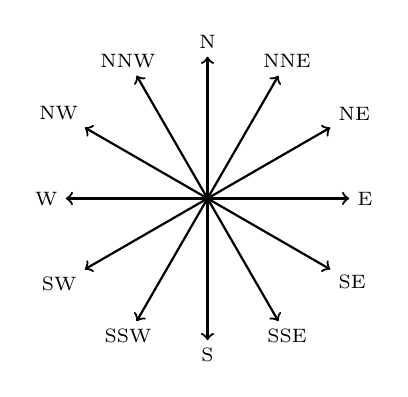
\begin{tikzpicture}
    \scriptsize
    \drawhex{0}{0}  
    \drawhex{0}{+1}  
    \drawhex{0}{-1}  
    \drawhex{+1}{+0.5}  
    \drawhex{+1}{-0.5}  
    \drawhex{-1}{+0.5}  
    \drawhex{-1}{-0.5}  
    \begin{scope}[thick,->]
        \draw (0,0) -- (0:1.8) node [anchor=180] {E};
        \draw (0,0) -- (30:1.8) node [anchor=210] {NE};
        \draw (0,0) -- (60:1.8) node [anchor=240] {NNE};
        \draw (0,0) -- (90:1.8) node [anchor=270] {N};
        \draw (0,0) -- (120:1.8) node [anchor=300] {NNW};
        \draw (0,0) -- (150:1.8) node [anchor=330] {NW};
        \draw (0,0) -- (180:1.8) node [anchor=0] {W};
        \draw (0,0) -- (210:1.8) node [anchor=30] {SW};
        \draw (0,0) -- (240:1.8) node [anchor=60] {SSW};
        \draw (0,0) -- (270:1.8) node [anchor=90] {S};
        \draw (0,0) -- (300:1.8) node [anchor=120] {SSE};
        \draw (0,0) -- (330:1.8) node [anchor=150] {SE};
    \end{scope}
    \drawaircraftcounter{0}{0}{60}{F-4}{}
\end{tikzpicture}
\end{fitwidth}



\AX{
\section{Facing}
\label{rule:facing}

Some elements also have a \emph{facing} that defines the direction in which they are pointed or traveling.

\paragraph{Principal Directions.}

The hex grid on the map defines twelve \emph{principal directions} from the center of each hex to the centers of its six sides and its six corners. Each principal direction differs from the adjacent principal directions by 30{\deg}.

The scenario will define the direction of north relative to the maps and the hex grid. It will always be aligned with one of the principal directions. Each principal direction is associated with a compass heading, as shown by Figure~\ref{figure:facing}.

\paragraph{Aircraft and Missiles.} 

The game counters representing aircraft and missiles must be oriented with their nose toward a principal direction. This direction defines their facing. 

If an aircraft or missile is located in a hex, it may potentially face toward any one of the principal directions (i.e., toward any of the sides or corners). If it is on a hex side, it must face in one of the two principal directions parallel to the hex side, as shown by Figure~\ref{figure:aircraft-map-location}.

\paragraph{Ground and Naval Units.}

The game counters representing heavy AAA units (see rule~\ref{rule:heavy-aaa-unit-facing}) and large naval units (see rule~\ref{rule:naval-units}) must be faced with their top or bow toward a principal direction. This direction defines their facing.

Other ground and naval units do not have defined facings, and the orientation of the counters representing them is not significant.
}


\addedin{2B}{2B-range}{
\section{Range}
\label{rule:range}

Many rules depend on the \emph{range} from one element to another. Other than in the exceptional cases noted subsequently, the range in hexes between two elements is determined as using the following procedure.

\paragraph{Range Procedure.}
The range has two components, the horizontal and vertical ranges. They are determined and combined as follows:

\begin{onecolumnfigure}[tb]

\begin{tikzfigure}{3.333\standardhexwidth}

    \drawhexgrid{0}{0}{2}{2}  

    \begin{athex}{0.50}{0.25}
        \drawdotathex[black!25]{+0.00}{0.50}
        \drawdotathex[black!25]{+0.00}{1.00}
        \drawdotathex[black!25]{+0.50}{0.25}
        \drawdotathex{+0.50}{0.75}
        \drawdotathex[black!25]{+0.50}{1.25}
        \drawdotathex[black!25]{+1.00}{0.50}
        \drawdotathex[black!25]{+1.00}{1.00}
    \end{athex}

    %\begin{athex}{3.50}{0.25}
    %    \drawdotathex[black!25]{+0.00}{0.50}
    %    \drawdotathex[black!25]{+0.00}{1.00}
    %    \drawdotathex[black!25]{+0.50}{0.25}
    %    \drawdotathex{+0.50}{0.75}
    %    \drawdotathex[black!25]{+0.50}{1.25}
    %    \drawdotathex[black!25]{+1.00}{0.50}
    %    \drawdotathex[black!25]{+1.00}{1.00}
    %\end{athex}
    
\end{tikzfigure}

\figurecaption{figure:range}{Range. The map locations shown in gray are one-half of a hex from the map location shown in black.}

\end{onecolumnfigure}


\begin{itemize}
\item
The \emph{horizontal range} is the length of the shortest route between the map locations, measured in hexes and counting only whole hexes.

If both elements are on hex centers, then the procedure is straightforward and probably familiar. However, if one or both are on hex sides, it may be less familiar. Figure~\ref{figure:range} shows map locations that are half a hex and one hex apart, including both hex centers and hex sides. These diagrams can be understood by noting that the distance from each map location to the surrounding six map locations is half a hex.

Figure~\ref{figure:range-example} gives examples of horizontal ranges.

\item
The \emph{vertical range} is the difference in altitude levels divided by two and rounded down. That is, each two whole altitudes levels of difference counts as one hex of vertical range.
\item
The \emph{range} is the sum of the horizontal and the vertical ranges.
\end{itemize}

\paragraph{Range Exceptions.}
The normal range procedure is \emph{not} used in the following cases:
\begin{itemize}

\item
The range for air-to-air gun attacks is determined according to rule~\ref{rule:air-to-air-gun-combat}.

\item
When attempting to search for a higher aircraft in daylight, the vertical range is the difference in altitude levels divided by \emph{four} and rounded down (see rule~\ref{rule:sighting-aircraft-and-missiles}).

\item
When considering positions of advantage, the horizontal range and vertical altitude difference are considered separately (see rule~\ref{rule:positions-of-advantage}).

\item
When determining if a radar target is in ground clutter, the horizontal range and vertical altitude difference are considered separately (see rule~\ref{rule:radar-ground-clutter}).

\end{itemize}

}

\addedin{2B}{pro}{

\paragraph{Closeness.}
\label{rule:closeness}

Range is used to determine relative closeness. If two aircraft have different ranges from a reference element, the one with the smaller range is considered to be closer to the reference element. If two aircraft have the same range, they are considered to be equally close. (That is, horizontal differences of half a hex and vertical differences of an odd number of altitude levels are ignored when determining closeness.)

For example, assuming all the aircraft in Figure~\ref{figure:range-example} have the same altitude, then aircraft C and D are equally close to aircraft A, since both are at a range of 2 hexes. Furthermore, assuming that aircraft A and C are at the same altitude and aircraft D is one altitude level below or above, then aircraft C and D are still equally close to aircraft A since both are still at a range of 2 hexes.

}

\section{Stacking}

\CX{
It is allowed, within the limits given below, for more than one counter to be in the same position on the map at the same time. When counters end up on top of other counters at the end of a turn, they are considered stacked. Stacking restrictions apply only al the end of a turn after all moves are completed.
}{
Counters are considered to be stacked when they occupy the same map location at the end of a game turn. Stacking is permitted within the limits given below. These limits only apply at the end of a game turn.
}

\CX{

\paragraph{In The Air.}
Aircraft and missiles may freely fly through hexes or hexsides containing other game counters. They may freely stack on top of ground and naval units. They may freely stack with other aircraft and missiles that are not at the same altitude level. However, no more than two friendly aircraft may safely end up stacked together at the same altitude level (unless in Close Formation). Aircraft from opposing sides may not stack together at the same altitude safely. If these last two situations occur, you must check for collisions.

Exception: Up to four aircraft may be stacked together and may safely fly together at the same altitude while in a close formation. See advanced Rule 5.6.

\paragraph{On The Ground.}
No more than four ground unit counters may ever stack in the same ground terrain hex. No more than four small naval unit counters may ever stack in the same water, coastal, or river terrain hex. No more than two large naval unit counters may ever stack in the same water hex. When taxiing on the ground, up to four aircraft may move together in a stack.

}{

\paragraph{Aircraft.} Aircraft in flight may stack with other aircraft, missiles, ground units, and naval units without limit. However, if aircraft in flight are stacked at the same altitude level, there may be a risk of collision according to rule~\ref{rule:aircraft-collisions}. No more than four aircraft may stack together when taxiing on the ground.

\paragraph{Missiles.} Missiles may stack with other missiles, aircraft, ground units, and naval units without limit.

\paragraph{Ground Units.} No more than four ground unit counters may be stacked in the same ground terrain hex. 

\paragraph{Naval Units.} No more than four small naval unit counters may be stacked in the same water, coastal, or river terrain hex. No more than two large naval unit counters may be stacked in the same water hex.

}

\AY[3A-angle-off]{

\section{Relative Position}

The relative position of one aircraft or missile with respect to another is crucial for many aspects of the air combat. For example, radars are typically restricted to scanning in a forward cone, the aircraft fuselage and wings can prevent the crew sighting to the rear and below, early infrared-homing missiles could only track targets from behind, and it is easier to compensate gunfire for deflection when firing from the rear or front of the target than from the beam.



% including air-to-air gun and rocket attacks (rule~\ref{rule:air-to-air-gun-combat}), air-to-air missile launches, tracking, and attacks  (rule~\ref{rule:air-to-air-missiles}), visual sighting (rule~\ref{rule:sighting-aircraft-and-missiles}), advantage (rule~\ref{rule:initiative}), and radar detection, tracking, and illumination (rule~\ref{rule:air-to-air-radar}).

In the game, the relative position can have two components: the horizontal relative position or angle-off arc (see rule \ref{rule:angle-off}) and the vertical relative position (see \ref{rule:vertical-limits}). 

\subsection{Reference and Distant Elements} To be clear in our terms, we will define the relative position of a \emph{distant element}  with respect to a \emph{reference element}. These roles depend on the context:

\begin{itemize}

\item In air-to-air gun, rocket, and missile attacks (rules~\ref{rule:air-to-air-gun-combat}, \ref{rule:air-to-air-rocket-combat}, and \ref{rule:missile-attacks}), the target aircraft is the reference element and the attacking aircraft or missile is the distant element.

\item For visual sighting (rule~\ref{rule:sighting-aircraft-and-missiles}), the sighting aircraft is the reference element and the aircraft or missile being sighted is the distant element.

\item For advantage (rule~\ref{rule:initiative}), the aircraft potentially in a superior position is the reference element and the aircraft potentially in an inferior position is the distant element.

\item For envelopes and IRM launch requirements (rules~\ref{rule:missile-launches} and \ref{rule:irm-launch-requirements}), the target aircraft is the reference element and the launching aircraft is the distant element.

\item When determining the field of view of sensors, the aircraft or missile sensing is the reference element and the aircraft being sensed is the distant element. Sensors include:
\begin{itemize} 
\item IRSTS (rule~\ref{rule:irsts}),
\item VAS (rule~\ref{rule:irsts}),
\item missile seekers (rule~\ref{rule:air-to-air-missiles}), and
\item air-to-air radar (rule~\ref{rule:air-to-air-radar}).
\end{itemize}


\item When determining the field of effect of jammers, the aircraft jamming is the reference element and the radar being jammed is the distant element.

\item When determining the field of laser designators (rule~\ref{rule:laser-guided-weapons}), the designating aircraft is the reference aircraft and the target is the distant element.

\end{itemize}

\subsection{Angle-Off Arcs}
\label{rule:angle-off}

%!TEX root = ../rules-working.tex
%LTeX: enabled=false

\silentlychangedin{1B}{1B-figures}{

\begin{twocolumnfigure}
\includegraphics[width=0.3\linewidth]{figures/figure-angle-off-facing-hex-side.pdf}
\includegraphics[width=0.3\linewidth]{figures/figure-angle-off-facing-hex-corner.pdf}
\includegraphics[width=0.3\linewidth]{figures/figure-angle-off-on-hex-side.pdf}
\end{twocolumnfigure}

}{

\begin{twocolumnfigure}[tbp]

\begin{minipage}[t]{0.33\linewidth}
\begin{fitwidth}{\linewidth}
\begin{tikzpicture}
    \tiny
    %setfiguresize{-4.1}{-5*\hexxfactor-0.1}{+4.1}{+5*\hexxfactor+0.1}
    %\setfiguresize{-4.67*\hexxfactor-0.1}{-4.5-0.1}{+4.67*\hexxfactor+0.1}{+4.5+0.1}
    \setfiguresize{-5.1}{-5.1}{+5.1}{+5.1}
    \begin{scope}
       \drawevenhexgrid{-5}{-4.5}{11}{10}
        \begin{scope}[dashed,very thick,->]
            \draw (0,0) --   (0:10);
            \draw (0,0) --  (30:10);
            \draw (0,0) --  (60:10);
            \draw (0,0) --  (90:10);
            \draw (0,0) -- (120:10);
            \draw (0,0) -- (150:10);
            \draw (0,0) -- (180:10);
            \draw (0,0) -- (210:10);
            \draw (0,0) -- (240:10);
            \draw (0,0) -- (270:10);
            \draw (0,0) -- (300:10);
            \draw (0,0) -- (330:10);
        \end{scope}
        \miniathex{+0.0}{+2.0}{\draw node [rotate=90, anchor=south] {\arcline{180} line};}
        \miniathex{+0.0}{-2.0}{\draw node [rotate=90, anchor=south] {\arcline{0} line};}
        \miniathex{+1.0}{-3.5}{\draw node {\minitable{c}{Right\\\arc{30}}};}
        \miniathex{+3.0}{-2.5}{\draw node {\minitable{c}{Right\\\arc{60}}};}
        \miniathex{+4.0}{-1.0}{\draw node {\minitable{c}{Right\\\arc{90}}};}
        \miniathex{+4.0}{+1.0}{\draw node {\minitable{c}{Right\\\arc{120}}};}
        \miniathex{+3.0}{+2.5}{\draw node {\minitable{c}{Right\\\arc{150}}};}
        \miniathex{+1.0}{+3.5}{\draw node {\minitable{c}{Right\\\arc{180}}};}
        \miniathex{-1.0}{+3.5}{\draw node {\minitable{c}{Left\\\arc{180}}};}
        \miniathex{-3.0}{+2.5}{\draw node {\minitable{c}{Left\\\arc{150}}};}
        \miniathex{-4.0}{+1.0}{\draw node {\minitable{c}{Left\\\arc{120}}};}
        \miniathex{-4.0}{-1.0}{\draw node {\minitable{c}{Left\\\arc{90}}};}
        \miniathex{-3.0}{-2.5}{\draw node {\minitable{c}{Left\\\arc{60}}};}
        \miniathex{-1.0}{-3.5}{\draw node {\minitable{c}{Left\\\arc{30}}};}

        \ifaids
            \drawaircraftcounter{0.00}{0.00}{90}{MiG-21}{}{}
        \else
            \drawaircraftcounter{0.00}{+0.00}{90}{MiG-21}{A}{1}
            \drawaircraftcounter{2.00}{-1.00}{150}{F-4}{B}{1}
            \drawaircraftcounter{3.00}{-0.50}{150}{F-4}{C}{1}
        \fi
    \end{scope}
\end{tikzpicture}
\end{fitwidth}
\ifaids\else
\par\bigskip

\begin{minipage}{0.8\linewidth}
A1 is the reference aircraft.

B1 is in the right \arc{60} arc.

C1 is in the right \arc{90} arc.

\end{minipage}
\fi
\end{minipage}
\hfil
\begin{minipage}[t]{0.33\linewidth}
\begin{fitwidth}{\linewidth}
\begin{tikzpicture}
    \tiny
    \setfiguresize{-5.1}{-5.1}{+5.1}{+5.1}
    \begin{scope}[rotate=90]
        \drawevenhexgrid{-5}{-4.5}{11}{10}
        \silentlychangedin{1C}{1C-apj-23-errata}{
            \node at (0,0) [draw,fill=white] {Diagram Incorrect in Original};
        }{
            \begin{scope}[dashed,very thick,->]
                \draw (0,0) --   (0:10);
                \draw (0,0) --  (30:10);
                \draw (0,0) --  (60:10);
                \draw (0,0) --  (90:10);
                \draw (0,0) -- (120:10);
                \draw (0,0) -- (150:10);
                \draw (0,0) -- (180:10);
                \draw (0,0) -- (210:10);
                \draw (0,0) -- (240:10);
                \draw (0,0) -- (270:10);
                \draw (0,0) -- (300:10);
                \draw (0,0) -- (330:10);
            \end{scope}
            \miniathex{+2.0}{+0.0}{\draw node [rotate=90, anchor=south] {\arcline{180} line};}
            \miniathex{-2.0}{-0.0}{\draw node [rotate=90, anchor=south] {\arcline{0} line};}
            \miniathex{+4.0}{+1.0}{\draw node {\minitable{c}{Left\\\arc{180}}};}
            \miniathex{+3.0}{+2.5}{\draw node {\minitable{c}{Left\\\arc{150}}};}
            \miniathex{+1.0}{+3.5}{\draw node {\minitable{c}{Left\\\arc{120}}};}
            \miniathex{-1.0}{+3.5}{\draw node {\minitable{c}{Left\\\arc{90}}};}
            \miniathex{-3.0}{+2.5}{\draw node {\minitable{c}{Left\\\arc{60}}};}
            \miniathex{-4.0}{+1.0}{\draw node {\minitable{c}{Left\\\arc{30}}};}
            \miniathex{-4.0}{-1.0}{\draw node {\minitable{c}{Right\\\arc{30}}};}
            \miniathex{-3.0}{-2.5}{\draw node {\minitable{c}{Right\\\arc{60}}};}
            \miniathex{-1.0}{-3.5}{\draw node {\minitable{c}{Right\\\arc{90}}};}
            \miniathex{+1.0}{-3.5}{\draw node {\minitable{c}{Right\\\arc{120}}};}
            \miniathex{+3.0}{-2.5}{\draw node {\minitable{c}{Right\\\arc{150}}};}
            \miniathex{+4.0}{-1.0}{\draw node {\minitable{c}{Right\\\arc{180}}};}
            \ifaids
                \drawaircraftcounter[90]{+0.00}{+0.00}{60}{F-105}{}{}
            \else
                \drawaircraftcounter[90]{+0.00}{+0.00}{0}{F-105}{A}{2}
                \drawaircraftcounter[90]{+1.00}{-0.50}{210}{MiG-21}{B}{2}
                \drawaircraftcounter[90]{-3.00}{-0.00}{0}{F-105}{C}{2}
            \fi
        }
    \end{scope}
\end{tikzpicture}
\end{fitwidth}
\ifaids\else
\par\bigskip
\begin{minipage}{0.8\linewidth}
A2 is the reference aircraft.

B2 is in the right \arc{150} arc.

C2 is on the \arcline{0} line.

\end{minipage}
\fi
\end{minipage}
\hfil
\begin{minipage}[t]{0.33\linewidth}
\begin{fitwidth}{\linewidth}
\begin{tikzpicture}
    \tiny
    \setfiguresize{-5.1}{-5.1}{+5.1}{+5.1}
    \begin{scope}[rotate=90]
        \drawoddhexgrid{-5}{-4.0}{11}{10}
        \silentlydeletedin{2B}{2B-angle-off-on-hex-side}{
            \begin{scope}[dashed,very thick,->]
                \miniathex{+0.333}{+0.000}{\draw (0,0) -- (300:10);}
                \miniathex{+1.000}{+0.000}{\draw (0,0) -- (330:10);}
                \draw (0,0) --  (0:10);
                \miniathex{+1.000}{+0.000}{\draw (0,0) --  (30:10);}
                \miniathex{+0.333}{+0.000}{\draw (0,0) --  (60:10);}
                \draw (0,0) -- (90:10);
                \miniathex{-0.333}{+0.000}{\draw (0,0) -- (120:10);}
                \miniathex{-1.000}{+0.000}{\draw (0,0) -- (150:10);}
                \draw (0,0) -- (180:10);
                \miniathex{-1.000}{+0.000}{\draw (0,0) -- (210:10);}
                \miniathex{-0.333}{+0.000}{\draw (0,0) -- (240:10);}
                \draw (0,0) -- (270:10);
            \end{scope}
        }
        \silentlyaddedin{2B}{2B-angle-off-on-hex-side}{
            \begin{scope}[dashed,very thick,->]
                \draw (0,0) --   (0:10);
                \draw (0,0) --  (30:10);
                \draw (0,0) --  (60:10);
                \draw (0,0) --  (90:10);
                \draw (0,0) -- (120:10);
                \draw (0,0) -- (150:10);
                \draw (0,0) -- (180:10);
                \draw (0,0) -- (210:10);
                \draw (0,0) -- (240:10);
                \draw (0,0) -- (270:10);
                \draw (0,0) -- (300:10);
                \draw (0,0) -- (330:10);
            \end{scope}        
        }
        \miniathex{+2.0}{+0.0}{\draw node [rotate=90, anchor=south] {\arcline{180} line};}
        \miniathex{-2.0}{-0.0}{\draw node [rotate=90, anchor=south] {\arcline{0} line};}
        \miniathex{+4.0}{+1.0}{\draw node {\minitable{c}{Left\\\arc{180}}};}
        \miniathex{+3.0}{+2.5}{\draw node {\minitable{c}{Left\\\arc{150}}};}
        \miniathex{+1.0}{+3.5}{\draw node {\minitable{c}{Left\\\arc{120}}};}
        \miniathex{-1.0}{+3.5}{\draw node {\minitable{c}{Left\\\arc{90}}};}
        \miniathex{-3.0}{+2.5}{\draw node {\minitable{c}{Left\\\arc{60}}};}
        \miniathex{-4.0}{+1.0}{\draw node {\minitable{c}{Left\\\arc{30}}};}
        \miniathex{-4.0}{-1.0}{\draw node {\minitable{c}{Right\\\arc{30}}};}
        \miniathex{-3.0}{-2.5}{\draw node {\minitable{c}{Right\\\arc{60}}};}
        \miniathex{-1.0}{-3.5}{\draw node {\minitable{c}{Right\\\arc{90}}};}
        \miniathex{+1.0}{-3.5}{\draw node {\minitable{c}{Right\\\arc{120}}};}
        \miniathex{+3.0}{-2.5}{\draw node {\minitable{c}{Right\\\arc{150}}};}
        \miniathex{+4.0}{-1.0}{\draw node {\minitable{c}{Right\\\arc{180}}};}
        \ifaids
            \drawaircraftcounter[90]{+0.0}{+0.00}{0}{MiG-21}{}{}
        \else
            \drawaircraftcounter[90]{+0.00}{+0.00}{0}{MiG-21}{A}{3}
            \drawaircraftcounter[90]{+0.00}{+1.50}{300}{F-4}{B}{3}
            \drawaircraftcounter[90]{-1.00}{+0.00}{30}{F-4}{C}{3}
        \fi
    \end{scope}
\end{tikzpicture}
\end{fitwidth}

\notein{2B}{New angle-off figure for 2B-angle-off-on-hex-side.}

\ifaids\else

\par\bigskip

\begin{minipage}{0.8\linewidth}
A3 is the reference aircraft.

B3 is in the left \arc{90} arc.

C3 is in the right \arc{30} arc (if it was facing A it would be on the \arcline{0} line).

\end{minipage}

\fi
\end{minipage}

\figurecaption{figure:angle-off}{Horizontal arcs.}

\end{twocolumnfigure}
}




%!TEX root = ../rules-working.tex
%LTeX: enabled=false

\begin{twocolumntablefloat}

\begin{twocolumntable}

\tablecaption{table:angle-off-borderlines}{Horizontal Arc Borderline Summary.}
\small
\begin{tabularx}{0.7\linewidth}{lLl}
\toprule
Context&First&Second\\
\midrule
Sensors&Included in the field.&---\\
Jammers&Included in the field.&---\\
Laser Designators&Included in the field.&---\\
Gun and Rocket Attacks&Move the faster element forward.&Use the narrower arc.\\
Blind and Restricted Arcs&Move the faster element forward.&Use the rearward arc.\\
Superior Position&Move the faster element forward.&Use the rearward arc.\\
Missile Launch Envelopes&Move the faster element forward.&Use the wider arc.\\
IRM Launch Target Aspect&Move the faster element forward.&Use the wider arc.\\
Missile Attacks&Move the faster element forward.&Use the wider arc.\\
\bottomrule
\end{tabularx}


\end{twocolumntable}

\vspace{\floatsep}

\begin{twocolumntable}

\tablecaption{table:angle-off-adjacent}{Wider, Narrower, and Rearward Horizontal Arcs.}

\small
\begin{tabularx}{0.7\linewidth}{CCCC}
\toprule
Borderline&Narrower Arc&Wider Arc&Rearward Arc\\
\midrule
\arcline{0}                                &\phantom{0}\arc{30}&\phantom{0}\arc{30}&\phantom{0}\arc{30}\\
\phantom{0}\arc{30} and \arc{60}\phantom{0}&\phantom{0}\arc{30}&\phantom{0}\arc{60}&\phantom{0}\arc{30}\\
\phantom{0}\arc{60} and \arc{90}\phantom{0}&\phantom{0}\arc{60}&\phantom{0}\arc{90}&\phantom{0}\arc{60}\\
\phantom{0}\arc{90} and \arc{120}\phantom{}&\phantom{0}\arc{90}&\phantom{}\arc{120}&\phantom{0}\arc{90}\\
\phantom{}\arc{120} and \arc{150}\phantom{}&\phantom{}\arc{150}&\phantom{}\arc{120}&\phantom{}\arc{120}\\
\phantom{}\arc{150} and \arc{180}\phantom{}&\phantom{}\arc{180}&\phantom{}\arc{150}&\phantom{}\arc{150}\\
\arcline{180}                              &\phantom{}\arc{180}&\phantom{}\arc{180}&\phantom{}\arc{180}\\
\bottomrule
\end{tabularx}

\end{twocolumntable}


\end{twocolumntablefloat}


\paragraph{Angle-Off.} 

The relative horizontal position of the distant element with respect to the reference element is quantified by the horizontal angle between two imaginary lines, one extending behind the tail of the reference element and the other between the reference element and the distant element. This is known as the \emph{angle off the tail} or simply the \emph{angle-off}. 

If the distant element is directly behind the reference element, the angle-off is \arc{0}, if it is directly on the beam, the angle-off is \arc{90}, and if is is directly in front, the angle-off is \arc{180}.

\paragraph{Angle-Off Arcs.} 

Angle-off is grouped into \emph{arcs} covering \arc{30} to the left or right of the target. Figure~\ref{figure:angle-off} show these arcs. The appropriate figure is used according to whether the reference element is in a hex facing a hex corner, in a hex facing a hex side, or on a hex side.

\paragraph{Borderline Procedure.} 

The distant element will often unambiguously be in an angle-off arc. However, sometimes it will be located on the borderline between two arcs. In these case, use the disambiguation procedure described below and summarized in Tables \ref{table:angle-off-borderlines} and \ref{table:angle-off-adjacent}.

In the context of the field of view of sensors, the field of effect of jammers, and the field of laser designators, if either or both of the adjacent arcs are within the field, the borderline is also considered to be within the field. (In other words, the fields include the borderlines.)

In others contexts, if the distant element is on the border between the two \arc{0} arcs or the two \arc{180} arcs, it is considered to be in the \arc{0} arc or \arc{180} arc. This rules does not specify whether aircraft falls in the left or right arcs, but this is never relevant for the game rules. 

% TODO: How do we disambiguate missile envelopes and IRM launch requirements? Included would work for the latter, but not for the former.

For the other borderlines, the procedure for determining the arc is more complex. Consider the speeds of the reference element and distant element at the start of the game turn:
\begin{itemize}
\item If the reference element is slower, the distant element is in the arc it would move into if it moved forward.
\item If the reference element is faster, the distant element is in the arc it would move into if the reference element moved forward.
\item If neither is faster or if the distant element remains on the borderline after one of the previous two cases (i.e., it is facing directly towards or away from the reference element), the resolution again depends on the context:
\begin{itemize}
\item For gun and rocket attacks (rule~\ref{rule:air-to-air-gun-combat}), the distant element (attacking aircraft) is considered to be in the narrower arc.
\item For missile attacks (rule~\ref{rule:missile-attacks}), the distant element (attacking missile) is considered to be in the wider arc.
\item For determining blind and restricted arcs (rule \ref{rule:sighting-aircraft-and-missiles}), the distant element (element being sighted) is considered to be in the rearward arc.
\item For determining advantage purposes (rule~\ref{rule:initiative}), the distant element (element potentially disadvantaged) is considered to be in the rearward arc.
\end{itemize}
\end{itemize}

The narrower arc is the arc further from the \arc{120} arc. The wider arc is the arc closer to the \arc{120} arc. The rearward arc is the arc closer to the \arc{30} arc.

Ground elements are always considered to be slower than any aircraft.

\paragraph{Same-Location Procedure}
If the reference and distant element are at the same map location (i.e., the same hex or hex side), the angle-off arc is the same as it would be if the distant element (i.e., the non-reference element) were moved backwards one hex.

Moving the distant element backwards would always leave it on a borderline facing the reference element and so  requires the use of the disambiguation procedure for borderlines described above.

\paragraph{Angle-Off Lines.} The imaginary lines extending behind and ahead of the reference element are the \arc{0} and \arc{180} lines, respectively. Although not formally arcs, these lines are at times treated as such. To count as being on one of these lines, the distant element must be on the borderline and facing directly along it towards the reference element. If they are on the line but not facing directly along it towards the target, they are considered in either the \arc{30} or \arc{180} arc but not on the \arc{0} or \arc{180} lines.

\paragraph{Angle-Off Examples.}

Consider Figure~\ref{figure:angle-off}, in which the aircraft A1, A2, and A3 are the reference elements and aircraft B1, B2,  B3, C1, C2, and C3 are distant elements. 

Aircraft C2 is unambiguously on the \arc{0} line, and C1 is unambiguously in the right \arc{90} arc, but the other attackers are on borderlines between two arcs. Aircraft C3 cannot be on the \arc{0} line as it is not facing the target, but it is in the \arc{30} arc.

\begin{itemize}

\item
In the context of the field of view of sensors or field of effect of jammers, distant elements on borderlines are considered to be in within the field if either or both of the adjacent arcs are within the field. B1 would be within the field only if either the right \arc{60} arc, the right \arc{90} arc, or both were within the field. B2 would be within the field only if either the right \arc{150} arc, the right \arc{180} arc, or both were within the field. B3 would be within the field only if either the left \arc{90} arc, the left \arc{120} arc, or both were within the field.

\item In other contexts, we need to consider the relative speeds of the reference and distant elements:

\begin{itemize}
\item
If the reference elements were slower than the distant elements, then B2 and B3 would be considered to be in the arcs into which they move if they moved forward: B2 would be in the right \arc{150} arc and B3 would be in the left \arc{120} arc.

\item
If the reference elements were faster than the distant elements, then B2 and B3 would be considered to be in the arcs into which they move if the reference element moved forward: B2 would be in the right \arc{150} arc and B3 would be in the left \arc{90} arc.

\item
If the reference element and the distant aircraft had the same speeds, then the context would determine whether B2 and B3 are considered to be in the narrower, wider, or rearward arc. The same procedure would be used for B1 regardless of the relative speeds, since B1 is facing along a borderline.

\begin{itemize}

\item For gun and rocket attacks, the distant elements are in the narrower arc, so B1 would be in the right \arc{90} arc, B2 in the right \arc{180} arc, and B3 in right \arc{90} arc.

\item For missile attacks (for which the distant elements would be missiles), the distant elements are in the wider arc, so B1 would be in the right \arc{120} arc, B2 in the right \arc{150} arc, and B3 in right \arc{120} arc.

\item For visual sighting and advantage, the distant elements are in the rearward arc, so B1 would be in the right \arc{90} arc, B2 in the right \arc{150} arc, and B3 in right \arc{120} arc.

\end{itemize}

\end{itemize}

\end{itemize}


\paragraph{Ranges of Angle-Off Arcs.}
\label{rule:ranges-of-angle-off-arcs}
Ranges of angle-off arcs are used for restricted or blind regions for sighting, sensor fields of view, and determining advantage. If a range is given as an arc followed by a plus sign, it consists of those arcs and all more forward arcs. If a range is given as an arc followed by a minus sign, it consists of those arcs and all more rearward arcs. Ranges specified in this way consist of both the left and right arcs.

For example, a blind arc given as $\arcrange{60}{-}$ consists the \arc{30} and \arc{60} arcs and a radar search field given as $\arcrange{150}{+}$ consists of the \arc{150} and \arc{180} arcs. 

\paragraph{Lower Angle-Off Arcs.}
\label{rule:lower-angle-off-arcs}
Restricted or blind regions for sighting are sometimes given as \arc{30}L, \arc{60}L, or \arc{180}L. These refer to the \arcrange{30}{-}, \arcrange{60}{-}, or \arcrange{180}{+} arc ranges, but only apply to distant elements at lower altitude.

For example, a restricted arc given as \arc{180}{L} refers to the \arc{180} arcs but only for distant elements at lower altitude. This might apply to an aircraft in which the view from the cockpit forward and downwards is obscured by the nose.

\section{Vertical Limits}
\label{rule:vertical-limits}

}

\section{Aircraft Collisions}
\label{rule:aircraft-collisions}

\CX{
Collisions are possible during the Flight Phase whenever an aircraft executes a head-on gun attack at range zero\addedin{1B}{1B-apj-36-errata}{ and the aircraft are at the same altitude}. Collisions are also possible at the end of \changedin{1B}{1B-apj-36-errata}{a game-turn}{the flight phase} in the following situations:
}{
\paragraph{Potential Collisions.}
Collisions are possible in the following situations:
}

\begin{itemize}
    \IAX{If an aircraft carries out a head-on gun attack at range 0 (see rule~\ref{rule:air-to-air-gun-combat}) on a target at the same altitude.}
    \item \CX{
    If an aircraft is stacked at the same altitude level with any enemy aircraft, and/or
    }{ 
    If an aircraft is stacked at the same altitude as an enemy aircraft after all aircraft have moved. However, aircraft in a tailing chain (see rule~\ref{rule:tailing-enemy-aircraft}) will not collide with each other.
    }
    \item \CX{
    If an aircraft is stacked \addedin{2B}{2B-stacking}{at the same altitude }with two or more friendly aircraft and not in Close Formation.
    }{
    If more than two friendly aircraft are stacked at the same altitude after all aircraft have moved and they are not in a close formation (see rule~\ref{rule:close-formations}).
    }
    \itemaddedin{2B}{2B-stacking}{If more than four friendly aircraft are stacked at the same altitude after all aircraft have moved, even if they are in a close formation.}
\end{itemize}

\CX{
\paragraph{Collision Resolution.} 
\addedin{2B}{2B-collisions}{Potential collisions resulting from head-on gun attacks are resolved immediately after the attack. Other potential collisions are resolved at the end of the flight phase.} For each potential collision, the player who last moved into the position must roll the die. On a roll of 1, his aircraft collides with one of the others. Determine which aircraft it collides with randomly. Both aircraft immediately roll on the 10 column of the Damage table to determine their damage.

\paragraph{Collision Exceptions:} There are \changedin{1B}{1B-apj-36-errata}{two}{three} exceptions to the Potential Collision rule.

\begin{itemize}
    \item An aircraft tailing another will not collide with that aircraft.
    \item An aircraft which is flying in close formation will not collide with other friendly aircraft in that formation.
    \itemaddedin{1B}{1B-apj-36-errata}{An aircraft that has already rolled for a collision for a head-on gun attack does not roll again for a collision \addedin{2B}{2B-collisions}{at the same position }again at the end of the flight phase.}
\end{itemize}

\notein{1B}{AWF: There is a clarification of the collision exceptions in the APJ 23 errata, but it seems to restate the original exceptions. I have not included it.}

}{
\paragraph{Collision Resolution Procedure.} 
If an aircraft carries out a head-on gun attack at range 0 and the same altitude, it immediately checks for a collision. The other cases are resolved at the end of the flight phase. Of the aircraft that could collide and which have not already checked for a collision at the same position (because of a head-on gun attack), the one that moved last checks for a collision. To check for a collision, roll the die. On a roll of 1, the aircraft collides with one of the others. Determine the other aircraft randomly. Both aircraft suffer damage from a weapon with an attack rating of 10 (see rule~\ref{rule:aircraft-damage-resolution}).
}

